\documentclass[12pt]{article}

\usepackage{amsmath}
\usepackage{amssymb}
\usepackage{enumerate}
\usepackage{enumitem}
\usepackage{booktabs}
\usepackage{csquotes}
\usepackage[margin=1.25cm]{geometry}
\usepackage{hyperref}
\usepackage{tabularx}
\usepackage{tikz}
\usepackage{tcolorbox}
\usepackage{colortbl}
\usepackage{graphicx}
\usepackage{algorithm}
\usepackage{algpseudocode}
\usetikzlibrary{patterns, shapes.geometric, positioning, bayesnet}

\usepackage{titling}
\setlength{\droptitle}{-7em}
\usepackage{titlesec}
\titlespacing\section{0pt}{12pt plus 4pt minus 2pt}{4pt plus 2pt minus 2pt}

\title{Job Training in the 70s}
\author{Jacob John, Michael Hartmann, Sai Ganesh Nellore, Shravan Srinivasan}

\begin{document}

\maketitle

\begin{tcolorbox}
\begin{quote} \centering \textit{``To what extent does job training enable socially and financially disadvantaged men to increase their income in the 1970s?"} \end{quote}
\end{tcolorbox}

\section{Code and documentation}

The following calculates the backdoor estimate using functions present in the \text{utils} folder, specifically, \href{https://github.com/cs396s24/Proj-Job-Training/blob/main/utils/backdoor_utils.py}{\tt{backdoor\_utils.py}} to apply linear regression and estimate the average treatment effect:
\begin{enumerate}[itemsep=-0.25em]
    \item \href{https://github.com/cs396s24/Proj-Job-Training/blob/main/prop/1_ipw_re78.ipynb}{\tt{1\_ipw\_re78}}: Uses the backdoor estimate to calculate the average treatment effect as the difference in revenues, $E[Re_{78}^{a=1} - Re_{78}^{a=0}]$.
    \item \href{https://github.com/cs396s24/Proj-Job-Training/blob/main/prop/2_bd_re78_re75.ipynb}{\tt{2\_bd\_re78\_re75}}: Uses the backdoor estimate to calculate the average treatment effect as the difference in incremental revenues, $E[(Re_{78} - Re_{75})^{a=1} - (Re_{78} - Re_{75})^{a=0}]$.
    \item \href{https://github.com/cs396s24/Proj-Job-Training/blob/main/backdoor/3_bd_u78.ipynb}{\tt{3\_bd\_u78}}: Uses the backdoor estimate to calculate the risk ratio of unemployment $\frac{E[U_{78}^{a=1}]}{E[U_{78}^{a=0}]}$. However, this approach is discarded as it does not provide a reliable estimate.
\end{enumerate}
The following notebooks calculate propensity estimates using functions from \href{https://github.com/cs396s24/Proj-Job-Training/blob/main/utils/prop_utils.py}{\tt{prop\_utils.py}}, to calculate propensities, and \href{https://github.com/cs396s24/Proj-Job-Training/blob/main/utils/strat_utils.py}{\tt{strat\_utils.py}}, to stratify and compute the causal estimate:
\begin{enumerate}[itemsep=-0.25em]
    \item \href{https://github.com/cs396s24/Proj-Job-Training/blob/main/prop/1_ipw_re78.ipynb}{\tt{1\_ipw\_re78}}: Applies Inverse Propensity Weighting (IPW) to calculate the average treatment effect as the difference in revenues, $E[Re_{78}^{a=1} - Re_{78}^{a=0}]$.
    \item \href{https://github.com/cs396s24/Proj-Job-Training/blob/main/prop/2_ipw_re78_re75.ipynb}{\tt{2\_ipw\_re78\_re75}}: Applies IPW to calculate the average treatment effect as the difference in incremental revenues, $E[(Re_{78} - Re_{75})^{a} - (Re_{78} - Re_{75})^{a'}]$.
    \item \href{https://github.com/cs396s24/Proj-Job-Training/blob/main/prop/1_strat_re78.ipynb}{\tt{1\_strat\_re78}}: Uses propensity scores to create strata and then estimate the causal risk difference ($E[Re_{78}^{a=1} - Re_{78}^{a=0}]$) within each stratum.
    \item \href{https://github.com/cs396s24/Proj-Job-Training/blob/main/prop/2_strat_re78_re75.ipynb}{\tt{2\_strat\_re78\_re75}}: Uses propensity scores to create strata and then estimate the causal risk differences ($E[(Re_{78} - Re_{75})^{a=1} - (Re_{78} - Re_{75})^{a=0}]$) within each stratum.
\end{enumerate}
The synthetic data generation is implemented in \href{https://github.com/cs396s24/Proj-Job-Training/blob/main/synthetic/synthetic.ipynb}{\tt{synthetic.ipynb}} and \href{https://github.com/cs396s24/Proj-Job-Training/blob/main/utils/synthetic_utils.py} {\tt{synthetic\_utils.py}} and has been slightly simplified compared to the update. 
Heterogeneous treatments effects are estimated with the Causal Tree Learn library in \href{https://github.com/cs396s24/Proj-Job-Training/blob/main/hte/hte.ipynb}{\tt{hte.ipynb}}.

\section{Estimation implementation (2 points)}

\subsection{Backdoor Estimate}

Recall our DAG with our confounders from our \textit{update} report below. We previously stated erroneously that a backdoor estimate was not possible because we could not block the paths from the treatment (\texttt{treat}) to the outcome (\texttt{Re78}). We are revising this estimate to state that we can calculate the average treatment effect via a backdoor estimate. Still, we must block an entire set of confounders, $Z = \{\texttt{education, re74, re75, black, hispanic, married}\}$ as it allows us to block all paths from the treatment to the outcome.

\begin{center}
\begin{tikzpicture}[scale=0.6, transform shape, >=stealth, node distance=2.7cm]
    \tikzstyle{obs} = [draw, very thick, circle, minimum size=1.2cm, inner sep=2pt]

     \begin{scope}
        \path[->, very thick]
            node[obs] (age) {$Age$}
            node[obs, right of=age] (race) {$Race$}
            node[obs, right of=race] (marital) {$Marital$}
            node[obs, right of=marital] (edu) {$Edu$}
            node[obs, below of=race] (re74) {$Re74$}
            node[obs, right of=re74] (re75) {$Re75$}
            node[obs, below of=re74] (treat) {$Treat$}
            node[obs, right of=treat] (re78) {$Re78$}

            (age) edge[red, bend right=45] (treat)
            (race) edge[red, bend right=45] (treat)
            (marital) edge[red, bend left=55] (treat)
            (edu) edge[red, bend left=45] (treat)
            (re74) edge[red] (treat)
            (re75) edge[red] (treat)
            
            (age) edge[green, bend right=35] (re78)
            (race) edge[green, bend right=65] (re78)
            (marital) edge[green, bend left=55] (re78)
            (edu) edge[green, bend left=45] (re78)
            (re74) edge[green] (re78)
            (re75) edge[green] (re78)
            (treat) edge[blue] (re78)

            (age) edge[blue, bend left=45] (marital)
            (age) edge[blue, bend left=45] (edu)
            (age) edge[blue] (re74)
            (age) edge[blue] (re75)

            (race) edge[blue, bend left=45] (marital)
            (race) edge[blue, bend left=45] (edu)
            (race) edge[blue] (re74)
            (race) edge[blue] (re75)

            (marital) edge[blue] (re74)
            (marital) edge[blue] (re75)

            (edu) edge[blue] (re74)
            (edu) edge[blue] (re75)

            (edu) edge[blue, bend right=35] (marital)
            (marital) edge[blue] (re74)
            (marital) edge[blue] (re75)
            ;
    \end{scope}
\end{tikzpicture}
\end{center}

The backdoor estimate works by controlling for confounding variables.  By adjusting for these confounders, the backdoor estimate aims to block all non-causal paths (or backdoor paths) between the treatment and the outcome, thereby isolating the direct causal effect of the treatment. Our backdoor estimate is as follows:
\begin{align}
E[Y^{a=1} - Y^{a=0}] = \frac{1}{N} \sum_i^{N} E[Y \mid A=1, Z_i] - E[Y \mid A=0, Z_i]
\end{align}
Where $Y$ can be either $Re_{78}^{a=1} - Re_{78}^{a=0}$ or $(Re_{78} - Re_{75})^{a=1} - (Re_{78} - Re_{75})^{a=0}$. Our backdoor algorithm is as follows, and can be found in \href{https://github.com/cs396s24/Proj-Job-Training/blob/main/utils/backdoor_utils.py#L45}{{\tt backdoor\_utils.py(\#46)}}.

\begin{algorithm}[H]
\caption{Estimate Causal Effect using Backdoor Linear Regression}
\begin{algorithmic}[1]
\Require Dataset $df$ with columns for treatment, outcome, and confounders

\State $results$ {\tt = []}
\State Get sorted unique values of $treatments$

\For{each value $a\_val$ in $treatments$}
    \State Select rows in $df$ where treatment equals $a\_val$
    \State Fit linear regression $model$ using {\tt smf.ols} on subsetted rows as $Y \sim Z$
    \State Predict outcome $y\_pred$ for all observations
    \State Append $\hat{y\_pred}$ to $results$
\EndFor

\State \Return $\hat{y\_pred}^{a=1} - \hat{y\_pred}^{a=0}$
\end{algorithmic}
\end{algorithm}

\subsection{Treatment parameter}

Without loss of generality, assume that the treatment has a linear relationship with the outcome. Consequently, the counterfactual risk difference, denoted as $\beta$, would increase proportionally with $\omega_A$, representing the parameter $a$ in the linear regression model. In practice, the relationship between the treatment and the outcome may not be perfectly linear. Recall using our backdoor estimate, we can represent it as a linear regression estimate:

\begin{align}
E[Y^{a=1} - Y^{a=0}] = \frac{1}{N} \sum_{i}^{N} [(\omega_0 + \omega_{A} \cdot 1 + \omega_{Z}Z) - (\omega_0 + \omega_{A} \cdot 0 + \omega_{Z}Z)] = \omega_{A}
\end{align}

The parameter estimate is implemented in \href{https://github.com/cs396s24/Proj-Job-Training/blob/main/utils/backdoor_utils.py#L7}{{\tt backdoor\_utils.py(\#7)}} as follows:

\begin{algorithm}[H]
\caption{Estimate Causal Effect using treatment parameter}
\begin{algorithmic}[1]
\Require Dataset $df$ with columns for treatment, outcome, and confounders

\State Fit a linear regression $model$ using {\tt smf.ols} on $Y \sim A + Z$
\State Extract the coefficient of the treatment variable, $\omega_{A}$

\State \Return $\omega_{A}$
\end{algorithmic}
\end{algorithm}

Our model parameters for our \texttt{smf.OLS} is given below. Based on this, our treatment effect is given as US\$ 860, which is $\omega_a$. Given our derivation above, the remaining parameters would get canceled out.

\begin{verbatim}
Intercept: 777.0  treat: 860.0     age: -81.5   education: 528.0    black: -543.0
hispanic: 2170.0  married: 1220.0  re74: 0.278  re75: 0.568
\end{verbatim}

\subsection{IPW}

IPW estimates the causal effect of a treatment by creating a \textit{weighted} dataset where the distribution of confounders is balanced between treated and control groups. By applying weights inversely proportional to the propensity scores (i.e., the probability of receiving the treatment given confounders), IPW aims to mimic the conditions of a randomized experiment, thus allowing for a more accurate estimate in an observational setting.

This estimate is implemented in \href{https://github.com/cs396s24/Proj-Job-Training/blob/main/utils/prop_utils.py#L5}{{\tt prop\_utils.py(\#5)}} as follows:

\begin{algorithm}[H]
\caption{Estimate Causal Effect using IPW}
\begin{algorithmic}[1]
\Require Dataset $df$ with columns for treatment, outcome, and confounders

\State $results$ {\tt = []}
\State Get sorted unique values of $treatments$
\State Fit logistic regression $model$ using {\tt smf.mnlogit} as $A \sim Z$
\State Predict \textit{propensity} scores using $model$
\State Calculate \textit{IPW} as the inverse of \textit{propensity}

\For{each value $a\_val$ in $treatments$}
    \State Select rows in $df$ where treatment equals $a\_val$
    \State Take means of \textit{outcome} weighted on \textit{}{IPW}
    \State Append $\hat{y\_pred}$ to \textit{results}
\EndFor

\State \Return $\hat{y\_pred}^{a=1} - \hat{y\_pred}^{a=0}$
\end{algorithmic}
\end{algorithm}

\subsection{Strata Matching}

Akin to the Dehejia paper, our strata matching method divides the dataset into equal-sized strata based on the propensity scores. Within each stratum, the treatment and control groups should have similar distributions of covariates. This balancing of covariates within strata mimics the randomization process, allowing us to use observational data. Our estimate is given as follows:

Within each stratum $k$, we calculate the difference in mean outcomes:

$\beta_{k} = E[Y^{a=1}_k - Y^{a=0}_k]$

and then take the weighted average using the weight, $w_k = \frac{n_{T_k}}{n_T}$

Our final estimate looks like this:
$E[Y^{a=1} - Y^{a=0}] = \sum_{k=1}^{K} w_k \beta_{k} = \sum_{k=1}^{K} \frac{n_{T_k}}{n_T} \left( E[Y^{a=1}_k] - E[Y^{a=0}_k] \right)$ Where, $T_k$ represents the $k$-th treatment group.

This estimate is implemented in \href{https://github.com/cs396s24/Proj-Job-Training/blob/main/utils/strat_utils.py#L5}{{\tt strat\_utils.py(\#5)}} as follows:

\begin{algorithm}[H]
\caption{Estimate Causal Effect using Stratification by Propensity Scores}
\begin{algorithmic}[1]
\Require Dataset $df$ with columns for propensity score, treatment, and outcome

\State Divide $df$ into $num\_strata$ strata based on \textit{propensity} using quantile cut via {\tt pd.qcut(df["propensity"], num\_strata)}

\For{each stratum in $num\_strata$}
    \State Subset the data $df$

    \If{$treated$ and $control$ $\ne \phi$}
        \State Calculate $treated\_outcome$ and $control\_outcome$ as mean of $outcomel$ in $treated$ and $control$ respectively
        \State Calculate $effect$ as $treated\_outcome - control\_outcome$
        \State Calculate $\beta_{k} = E[Y^{a=1}_k - Y^{a=0}_k]$
    \EndIf
\EndFor

\State Calculate $overall\_effect$ as weighted average of $strata\_effects$
\State \Return $E[Y^{a=1} - Y^{a=0}]$
\end{algorithmic}
\end{algorithm}

\section{Changes since the update}

As mentioned in the previous section, we now have IPW and Backdoor estimates, which were previously unavailable. To ensure robust causal inference, blocking every confounder in our DAG is crucial to block all paths from treatment to the outcome. This allowed us to regress our confounders and treatment to predict the outcome. Specifically, we created individual linear models for each treatment, similar to our approach in homework assignments. This allowed us to capture non-linear relationships using existing linear models.

Despite these efforts, our initial estimates based solely on Revenue in 1978 were unsatisfactory. When running the estimates on the observational data, the average risk difference was negative, contrary to the experimental data indicating that job training is effective. Consequently, we updated the average treatment effect to reflect the difference in revenue increments from 1975 to 1978 (i.e., $Re_{78} - Re_{75}$).

To understand why this adjustment was necessary, consider the following table, which can also be found in the code \href{https://github.com/cs396s24/Proj-Job-Training/blob/main/prop/1_ipw_re78.ipynb}{here}. It illustrates how specific rows with higher IPW weights are misrepresenting our treatment group:

\begin{table}[h]
\centering
\begin{tabular}{|c|c|c|c|c|c|c|c|c|c|}
\hline
\texttt{black} & \texttt{hispanic} & \texttt{married} & \texttt{nodegree} & \texttt{treat} & \texttt{n} & $\hat{\texttt{ipw}}$ & $\hat{\texttt{re}_{78}}$ & $\hat{\texttt{re}_{75}}$ & $\hat{\texttt{re}_{78}} - \hat{\texttt{re}_{75}}$ \\
\hline
1 & 0 & 1 & 1 & 1 & 23 & 313.04 & 7050.81 & 3363.42 & 3687.38 \\
1 & 0 & 1 & 0 & 1 & 6 & 257.49 & 12183.93 & 4767.81 & 7416.11 \\
0 & 0 & 1 & 0 & 1 & 2 & 29.20 & 6209.05 & 426.86 & 5782.18 \\
... & ... & ... & ... & ... & ... & ... & ... & ... & ... \\
0 & 1 & 0 & 0 & 0 & 3 & 3.64 & 13090.19 & 7781.93 & 5308.25 \\
... & ... & ... & ... & ... & ... & ... & ... & ... & ... \\
1 & 0 & 0 & 1 & 0 & 73 & 2.31 & 8705.50 & 8457.18 & 248.32 \\
0 & 1 & 0 & 1 & 0 & 3 & 1.88 & 2709.16 & 1253.22 & 1455.93 \\
\hline
\end{tabular}
\caption{Rows with higher IPW misrepresenting the outcome.}
\label{tab:high_weightage}
\end{table}

We can see that these rows in table \ref{tab:high_weightage} represent a bulk of our means for the treatment and the non-treatment groups. While this does alleviate confounding, it skews the earnings to a lower value for the treatment group and a higher value for the non-treatment group. We could say that this might be due to job training, but upon closer look, we can see that the difference in revenue for the treatment group is much higher ($\hat{\texttt{re}_{78}} - \hat{\texttt{re}_{75}}$) as shown in figure \ref{fig:rev1975_78}. This tells us that the non-treatment group (in the observable data) typically started with a higher income in 1974, indicating some selection bias. We could work on mitigating this selection, but due to \textit{limited resources}, we are more interested in knowing whether training would help.

\begin{figure}
    \centering
    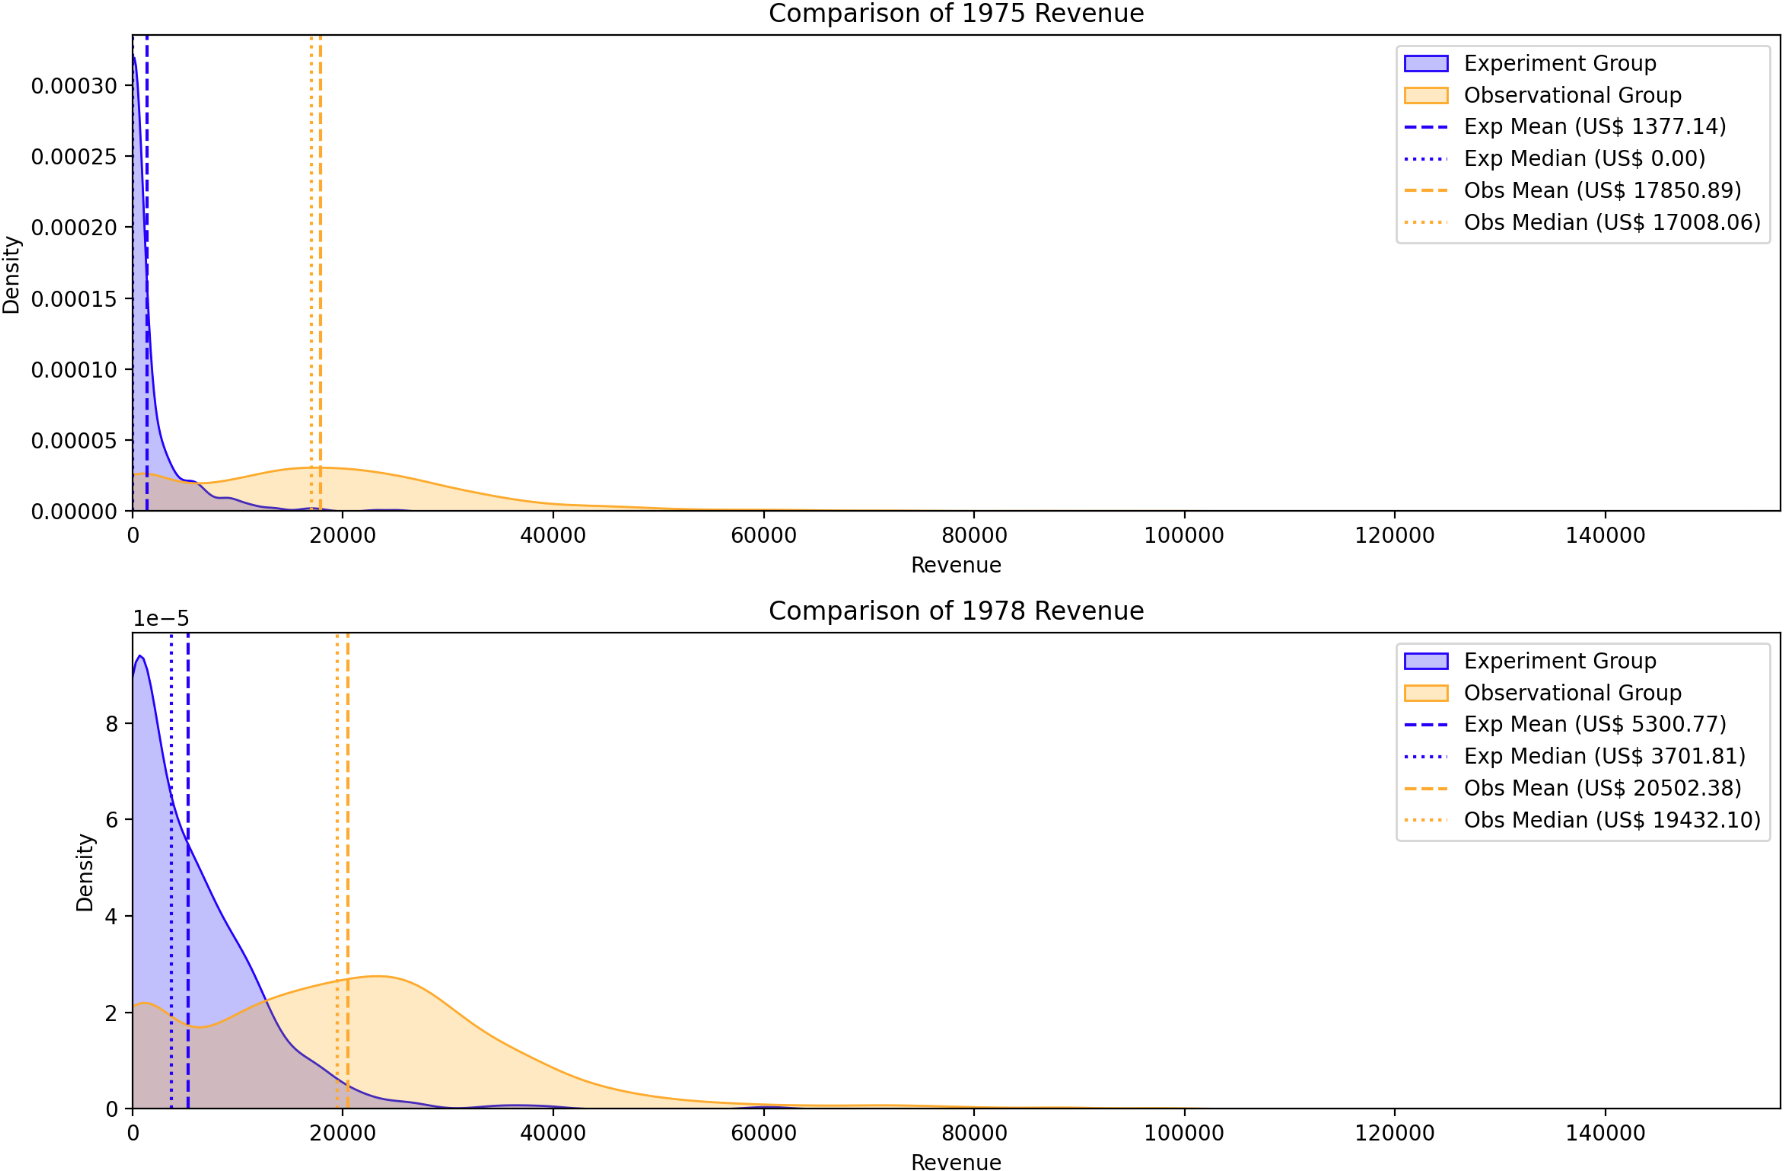
\includegraphics[width=0.7\linewidth]{rev1975_78.png}
    \caption{Comparing the Revenues of 1978 and 1975 between the experiment and treatment groups}
    \label{fig:rev1975_78}
\end{figure}

Therefore, it is advisable to consider the risk difference as it better reflects the policy goal of increasing revenue for individuals rather than just comparing their final revenue to those who did not receive training. We aim to see an increased benefit for those without wages, as the program seeks to assist the disadvantaged. Furthermore, (we assume) policymakers would have more reason to support those in need than those already well-off. This is because job training should be targeted towards individuals with no prior background, as those with a higher starting revenue already have some work experience.

We also started using a bootstrapped estimate to calculate confidence intervals. This approach allows us to determine whether our estimate is due to chance and provides a confidence interval. The bootstrap estimator, provided \href{https://github.com/cs396s24/Proj-Job-Training/blob/main/utils/bootstrap.py}{here}, allows us to check the robustness of our estimator:

\begin{itemize}[itemsep=-0.25em]
    \item We conduct {\tt num\_exp} experiments each with {\tt n} bootstrap samples.
    \item Assess the width of the confidence interval to understand the variability or precision of our estimator.
    \item Running multiple experiments helps check the consistency of our estimator.
    \item Use synthetic data to compare the mean of our bootstrap experiments to the known true value to check for bias in our estimate.
\end{itemize}

In our previous approach, we conducted our experiment across multiple strata and concluded the analysis without delving deeper. This time, however, we are focusing on minimizing the number of strata to better understand what each stratum represents. Our goal is not necessarily to achieve an unbiased estimate, but rather to obtain one with lower variance and higher reliability. Based on the feedback received, we are shifting our focus away from merely matching the observational estimate to the experimental one. Instead, we aim to understand the reasons behind the estimates produced and the rationale for grouping certain individuals based on their propensities.

We adapt the example code for binary treatments from the \href{https://github.com/edgeslab/CTL/tree/master}{CTL github repository} and run an HTE analysis on the observational data. Specifically, we use the difference between $re_{78}$ and $re_{75}$ as an outcome variable and all other columns except ``treat", ``nodegree", ``u75" and ``u74" (which are a function of the respective continuous variables) as covariates. We also experimented with using $re_{78}$ as an outcome, but the results were mostly very negative numbers - which we assume is due to a higher baseline income level in the untreated group.

Finally, we also decided to drop the risk ratio as we were seeing very poor results \href{https://github.com/cs396s24/Proj-Job-Training/blob/main/backdoor/3_bd_u78.ipynb}{here}. In the interest of time, we felt other methods were more fruitful.

\section{Interpreting results}

\begin{table}[h]
\centering
\begin{tabular}{|c|c|c|c|c|}
\hline
\textbf{Estimate} & \textbf{Method} & \textbf{Estimate} & \textbf{Lower CI} & \textbf{Upper CI} \\
\hline
$Re_{78}$ & RCT & 1796.24 & 522.92 & 3114.44 \\
$Re_{78} - Re_{75}$ & RCT & 1582.83 & 49.59 & 3126.33 \\
$Re_{78}$ & Backdoor LR & -9200.54 & -15795.52 & -2132.38 \\
$Re_{78} - Re_{75}$ & Backdoor LR & -9200.54 & -15795.52 & -2132.38 \\
\rowcolor{lightgray} $Re_{78}$ & Treat parameter & 861.24 & -549.37 & 2379.72 \\
\rowcolor{lightgray} $Re_{78} - Re_{75}$ & Treat parameter & 861.24 & -549.37 & 2379.72 \\
$Re_{78}$ & IPW & -14694.36 & -22000.2 & 1574.92 \\
\rowcolor{lightgray} $Re_{78} - Re_{75}$ & IPW & 2000.23 & -16544.84 & 20828.44 \\
$Re_{78}$ & Strata-Matching & -146.24 & -1720.24 & 1469.72 \\
\rowcolor{lightgray} $Re_{78} - Re_{75}$ & Strata-Matching & 1122.41 & -143.7 & 2300.95 \\
\hline
\end{tabular}
\caption{Estimates and Confidence Intervals by Method}
\label{tab:estimates_ci}
\end{table}

Table \ref{tab:estimates_ci} shows us the different methods and their estimates along with 95\% Confidence Interval. The first two are results from the RCT on the experimental data; the remaining are run using the observational data. Favorable results are highlighted.

\subsection{Backdoor estimate}

\subsubsection*{Before vs. After}

As previously mentioned, we did not conduct the backdoor estimate because we believed it was not feasible. We now know it is possible, as we can block on all confounders.

\subsubsection*{Interpretation}

We hypothesized that using the difference between revenues instead of the final revenue would improve our results with the backdoor estimator. However, this approach did not yield better results. Even with a pseudo-nonlinear model, our backdoor estimate failed to predict a positive estimate for the observable data. This outcome is due, in part, to the fact that when modeling our confounders, the differences in estimates using linear regression effectively cancel out, leading to the same outcome. This method produces a high variance and generally poor estimate, making it unsuitable for our policy. We hypothesize this method isn't working due to unobserved confounding or because the relationship between the variables cannot be adequately approximated with the linear model.
\subsection{Treatment Parameter}

\subsubsection*{Before vs. After}

This was a new approach we tried based on a derivation in the previous sections.

\subsubsection*{Interpretation}

Using the treat parameter yields a higher variance estimate compared to the backdoor method, but it is more unbiased (closer to the true estimate). We suspect this is because our model now includes the treatment variable, allowing it to capture the relationship with the outcome better. Interestingly, this estimate suggests that, based on observable data, individuals who receive job training would earn US\$861.24 more than those who do not, assuming all other factors are equal. However, the high variance means we cannot confidently assert this result. Ironically, we know this is accurate based on our experimental data. Nevertheless, relying solely on observational data, this result appears promising. Still, it would be premature to base policy decisions on it without considering heterogeneous treatment effects (HTEs) or addressing potential selection bias.

\subsection{IPW}

\subsubsection*{Before vs. After}

Our previous IPW estimate on the observable data using the $Re_78$ estimate produced very poor results. In the \textit{changes} section, we have delved into the motivation for using $Re_78—Re_75$.

\subsubsection*{Interpretation}

Using the difference-of-difference approach, we observe that IPW produces a promising estimate despite having a very high variance. As mentioned in the previous section, we cannot recommend a policy based solely on this high variance estimate. Since IPW inherently has high variance, we should consider applying clipping based on domain expertise in future works. However, it is essential to note that clipping may introduce a slight bias in the estimate.

\subsection{Strata Matching}

\subsubsection*{Before vs. After}

We attempted to align our observable estimate with our experimental one in our previous update. This approach revealed that using many strata could yield a better estimate. However, we did not determine the variance of this estimate since we did not perform bootstrapping. Our current goal is to identify a more interpretable number of strata and use it to analyze different stratum groups. Given time constraints, we will not pursue this. Instead, we will focus on using Heterogeneous Treatment Effects (HTEs) to understand where the effect is most pronounced.

\subsubsection*{Interpretation}

This method has the lowest variance and is the most unbiased. We found, through experimentation, that the lowest number of strata for an relatively unbiased estimate would be 7. However, since the lower confidence interval is still negative, we cannot confidently recommend a policy based on this job training data alone.

\subsection{Heterogeneous Treatment Effects}
\begin{figure}
    \centering
    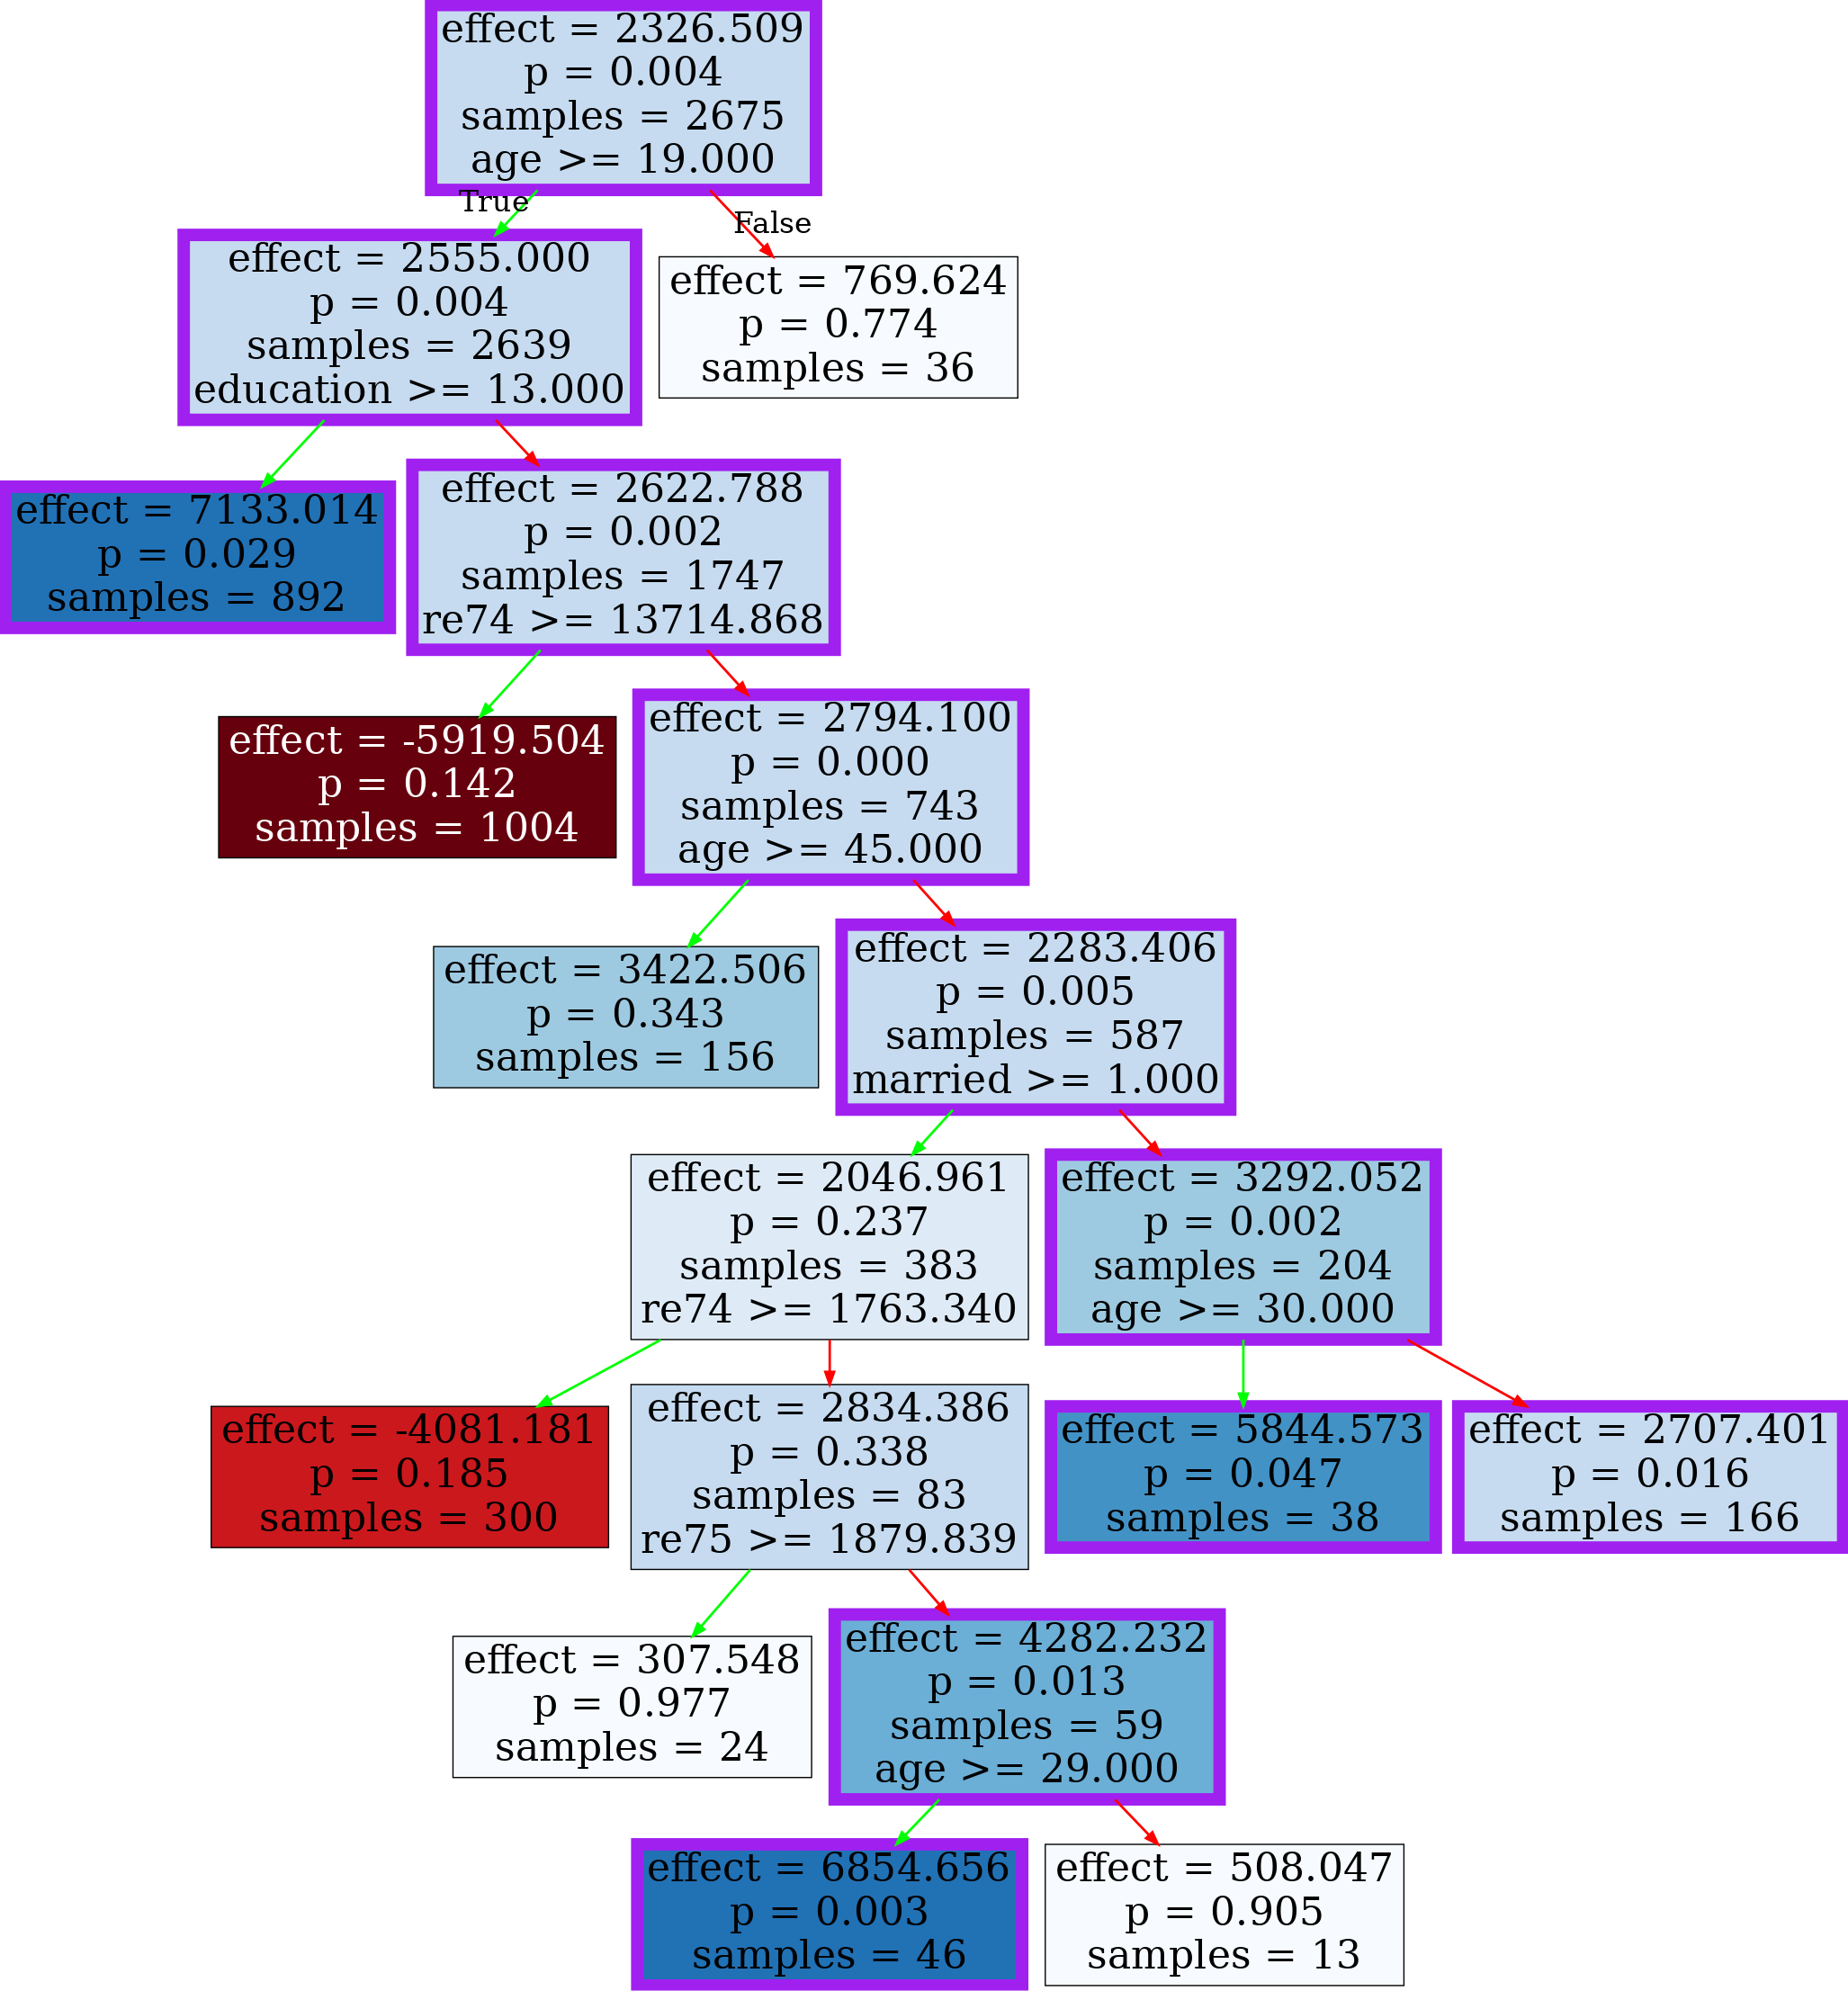
\includegraphics[width=0.5\linewidth]{bin_tree.png}
    \caption{Heterogeneous treatment effects on observational data (effect of treatment on the increase in earnings over study period) }
    \label{fig:hte}
\end{figure}

The tree we obtained using Causal Tree Learn on the observational data (using $re_{78}$ - $re_{75}$ as the outcome) is shown in figure \ref{fig:hte}. It seems to indicate that the group benefiting most (+\$7133) from job training is 19 years and older with at least 13 years of education. However, the tree indicates that the training has a strong negative effect (-\$5920) for people in the same age bracket with lower education (\textless 13 years) and high earnings in the year before the study ($re_{74} > 13715$). While the p-value is higher here, this applies to over 1000 people in the data. Assuming this effect is correct, we could speculate that these are employable individuals who possibly lost their jobs recently. They might see their earning potential reduced by taking a ``break" from the regular job market by doing the training.

Let's look at another interesting subgroup with low earnings in 1974 (\textless \$13715), younger than 45 and with less than 13 years of education. Among them, the largest effects are seen in the unmarried, middle-aged (30-45 years) subgroup (+\$5845) and in the similarly aged (29-45 years), married group with very low earnings in both 1974 and 1975 (\textless \$1763 and \textless \$ 1880 respectively) who see an average increase of \$6855.
Both of these groups are relatively small (38 and 46 individuals) but also have low p-values.

Tying this back to our causal questions, the CATEs allow us to make much more specific statements about who the treatment would likely be most and least helpful for and could inform more targeted recruitment strategies for such programs. The p-values give us an idea about how confident we can be about the groups and could be used to reflect on how to treat individuals who lie at the extreme ends of a group.  

\section{Synthetic Data}

We simplified the data-generating process from the update by removing ``nodegree" and estimating education in the same way as we did for the other continuous variables. Our simplified causal graph becomes:

% Node styles
\tikzstyle{circle}=[fill=white, draw=black, shape=circle, minimum height=1.5 cm, thick, font=\ttfamily]

% Edge styles
\tikzstyle{arrow}=[->, blue]

\begin{center}
\begin{tikzpicture}[scale=0.6, transform shape]
		\node [style=circle] (0) at (3, 2) {black};
		\node [style=circle] (1) at (6.75, 0.25) {treat};
		\node [style=circle] (4) at (0.25, -1.25) {age};
		\node [style=circle] (5) at (5, -1.25) {edu};
		\node [style=circle] (6) at (0.5, 2.5) {re74};
		\node [style=circle] (7) at (0.25, 0.75) {re75};
		\node [style=circle] (8) at (6.25, 2.25) {re78};
		\node [style=circle] (9) at (-1.75, 0) {married};
		\node [style=circle] (11) at (3, -0.5) {hisp};
		\draw [style=arrow] (0) to (4);
		\draw [style=arrow] (0) to (5);
		\draw [style=arrow] (0) to (6);
		\draw [style=arrow] (0) to (7);
		\draw [style=arrow] (0) to (8);
		\draw [style=arrow] (4) to (9);
		\draw [style=arrow] (5) to (1);
		\draw [style=arrow] (1) to (8);
		\draw [style=arrow] (0) to (1);
		\draw [style=arrow] (11) to (4);
		\draw [style=arrow] (11) to (5);
		\draw [style=arrow] (11) to (6);
		\draw [style=arrow] (11) to (7);
		\draw [style=arrow] (11) to (8);
\end{tikzpicture}
\end{center}
\texttt{black} and \texttt{hispanic} are generated as categorical variables following the distribution found in the observational data. Group statistics (mean, variance) are computed for the earning variables, age and education from the observational data which are used to sample these continuous variables from a multivariate Gaussian.
The binary treatment variable is sampled from a coin flip whose success probability is computed as  \texttt{0.25 +  (education >= 12) * 0.25 + black * 0.25}.
For the treated individuals, we then add a sample from another Gaussian ($\mu = 5000, \sigma = 500$). This means that despite the confounding, the causal effect of \$5000 is very simple to see (similar to the synthetic coin-flip data we saw in the lecture).

\begin{table}[h]
\centering
\begin{tabular}{|c|c|c|c|c|}
\hline
\textbf{Method} & \textbf{n} & \textbf{Estimate} & \textbf{Lower CI} & \textbf{Upper CI} \\
\hline
Naïve & 1000 & 4420.95 & 3393.72 & 5395.73 \\
Naïve & 10000 & 5004.29 & 4594.87 & 5358.68 \\
Naïve & 100000 & 5287.46 & 5165.69 & 5397.89 \\
Treat parameter & 1000 & 4480.77 & 3688.66 & 5340.47 \\
Treat parameter & 10000 & 4792.46 & 4480.72 & 5253.59 \\
Treat parameter & 100000 & 4984.9 & 4863.41 & 5083.52 \\
Strata-Matching & 1000 & 4356.52 & 3177.33 & 5391.32 \\
Strata-Matching & 10000 & 4717.56 & 4307.82 & 5068.4 \\
Strata-Matching & 100000 & 4913.45 & 4773.73 & 5030.68 \\
\hline
\end{tabular}
\caption{Estimates and Confidence Intervals by Method and Sample Size}
\label{tab:method_estimates}
\end{table}

Using our treat parameter and strata-matching ({\tt num\_strata = 7}) methods, we obtained our synthetic data results in Table \ref{tab:method_estimates}. Our naïve method ($E[Y \mid A]$) might be biased as it does not account for confounding. We observe that the estimate gets closer with {\tt n=10000} but deteriorates with a larger sample size, suggesting that the apparent accuracy at {\tt n=10000} might be due to chance. The naïve method produces a low variance estimate because it is a simple subtraction but fails to capture the true underlying relationships. In contrast, while having a higher variance, our other methods are more unbiased as they account for confounding variables.

\section{Reflections}

\subsection*{What was interesting?}
We were able to spend some more time on HTEs than was possible in the lecture. This was cool because the CTE package directly gave us a well-interpretable visual output, pointed out which variables are relevant, and was an interesting way to approach our dataset.

Researching the LaLonde and Dehejia papers also gave us a perspective on how the terminology has changed over time and which methods (e.g., stratified matching based on propensities) could be promising to try.
From the lecture, the standard IPW and backdoor estimators were probably the most relevant, along with the use of one parameter from a linear model for estimating the causal effect. Furthermore, it also helped us to understand what the data generation process was and what was meant by the Dehejia subset. It's interesting to see how the dataset online is commonly miscited as the LaLonde dataset, while in reality, it is the Dehejia subset of the LaLonde dataset. This is important as the subset only applies to disadvantaged male individuals as opposed to a larger population (thereby limiting the scope of this study).

\subsection*{What was difficult?}

Translating between the language in the Lalonde papers and the terminology we use in our course was a challenge that we could address with Prof. Zach's help. Working with the papers also helped us learn more about how the data was generated. 

While implementing the estimators from scratch is certainly a good learning experience, it made the code more verbose. Given that we already had the chance to do this in HW2, it might have been useful to learn to use doWhy to avoid careless mistakes and focus more on the estimates.

One significant challenge was the search for a suitable dataset. The availability of high-quality, complete datasets seems limited in many domains, so we recommend paying more attention to these aspects when choosing the causal question. We also stuck with sub-optimal datasets for too long and finally made the pragmatic choice of using a dataset known to work well with causal inference. This had the advantage of allowing us to focus more on the methods than preprocessing data but meant that it felt less like we were extracting new or unexpected insights from a dataset.


\subsection*{Unaddressed challenges}

There is very likely selection bias and some kind of unobserved confounding, which we did not address in our analysis and which might also be hard to quantify/infer from the columns in the data. That is, the treated group in the observational dataset might be entirely different kinds of people in ways not captured by simple demographic attributes and react differently to the training than the general population would. For example, someone's mental state or their previous years in jail/harshness of crime might also impact job training success. 

The specification of our statistical models could also impact the biases of our causal estimates. We use simple linear models to capture the relationships (including the one between the confounders and treatment). For example, we're assuming age has a linear influence on the outcome, which does not seem plausible (as also suggested by our HTE analysis). So even if our causal graph was a perfect representation of the real world, our estimate would still be biased if the actual relationship is more complex (which is likely).

We think selection bias is the more fundamental issue here because the variables available are quite coarse-grained and maybe a simple model can capture a lot of what is possible to extract from what we know about each individual. The selection bias present here might be a result of the fact that experienced professionals are unlikely to take job training - as one might expect, the individuals in the untreated group have a higher income to begin with. We suspect that accounting for work experience in this model might lead to better estimates, but we don't have access to those.

Finally, we don't present a rigorous argument for why some of the methods work better and for why the differences work better than the actual revenue. It would be interesting to find out why just using a parameter from the linear model gives so much more plausible results than a backdoor. Our suspicion stems from the fact that we're also accommodating for treatment, but we're not certain why this might be the case.

\subsection*{What's left to do?}

A promising next step would be performing a sensitivity analysis to quantify the influence the challenges outlined above would have on the quality of our estimates. 

The funding could be used to run a long-term randomized trial to obtain results applicable to a job market shaped by automation and increasingly AI. Job training would have to take different forms and have different effects compared to decades ago. Due to the massive technological advancements which have taken place in the meantime, today's job training would have to reflect this new environment to create an impact. The same approach of using additional observational data could help to identify potentially promising sections of the population where job training could be effective.

We should also check how this impacts jail recidivism. Since most of the people in this dataset are those from socially disadvantaged backgrounds, we would like to see how job training would affect their likelihood of going back to jail. Our hypothesis here is given a \textit{second} chance, inmates are less likely to commit crimes as more is at stake. Such an estimate would also be easier to sell to policymakers as this would be in the interest of public safety and not economics alone. 

Such insights could be generated from Northwestern's "Second Chance" program by measuring the impact of placing inmates into specific academic degrees.

\end{document}